% !TeX spellcheck = es_ES
\documentclass[twocolumn]{article}
\usepackage[spanish,mexico]{babel}



\usepackage{ieeetrantools}
\usepackage{mathtools}
%%%%%%%%%%%%%%%%%%%%%%
% TABULAR LINEBREAKS %
%%%%%%%%%%%%%%%%%%%%%%
\usepackage{makecell}



\renewcommand\theadalign{bc}
\renewcommand\theadfont{\bfseries}
\renewcommand\theadgape{\Gape[4pt]}
\renewcommand\cellgape{\Gape[4pt]}

%%%%%%%%%%
% MACROS %
%%%%%%%%%%
\newcommand{\adm}{\text{adm}}
\newcommand{\str}{\text{str}}
\newcommand{\Dext}{D_\text{ext}}
\newcommand{\Dint}{D_\text{int}}
\newcommand{\Pext}{P_\text{ext}}
\newcommand{\grad}{\ensuremath{^\circ \textrm{C}}}

\usepackage[symbol*]{footmisc}
\usepackage{titlesec}
\titleformat*{\section}{\normalfont\large\bfseries}
\titleformat*{\subsection}{\normalfont\normalsize\bfseries}

\title{Instalaciones Industriales}
\author{Hoja de formulas}
\date{\today}
\begin{document}
	\maketitle
	
	\tableofcontents
%{ \centering \vspace{-1cm}\par
%	{\Large Hoja de Formulas \par}
%	\vspace{.3cm}
%	{Instalaciones industriales\par}
%}
\section{Dise\~no de Ca\~ner\'ias de proceso[ASME B31.3]}
Esta norma es para caños de acero. Para caños de acero inoxidable se puede usar ASME B36.19. Cañerías de potencia ASME B31.1. ASME B16.9 rige para accesorios de cañerías.

Estimación de schedule: Sch$\approx 1000\cdot  \frac{P_d}{S}$ donde $S$ es el basic allowable stress.

El diámetro se puede calcular con la velocidad $v$ y el caudal deseado $Q$ del flujo interno.

El espesor mínimo permisible de la pared de un caño:
\[
t_{\min} = t_n+c
\]
corregido por tolerancias mecánicas del fabricante:
\[
t_{\text{elegido}} = \frac{t_{\min}}{0,875} = \frac{t_{n} + c}{0,875}
\]

donde $t_n$ es el espesor nominal calculado por la presión de diseño y $c$ incluye el sobre-espesor por corrosión y suma de geometrías mecánicas como profundidad de rosca. El 0,875 toma en cuenta una variación de 12,5\% de tolerancias mecánicas de fabricante.

\[
\text{Para } t<D/6:\quad t_{n} = \frac{P_d\cdot D}{2(S E W + Y \cdot P_d)}
\]
\begin{itemize}
	\item[$D$:] Diámetro nominal exterior en mm
	\item[$P_d$:] Presión de diseño interna en MPa
	\item[$S$:] Tensión admisible a temperatura $T_d$ (\textit{Basic allowable stress}
	\item[$E$:] Factor calidad de soldadura [A1-A, A1-B]
	\item[$W$:] Factor reducción de resistencia en la junta de soldadura [302.3.5]
	\item[$Y$:] Coeficiente Y (según material) [304.1.1]
\end{itemize}

La verificación ante presión externa se hace según ASME Section II (ver sección \ref{sec:asmeii}).

\subsection{Prueba hidrostática}
El fluido usado para la prueba será agua a menos que exista posibilidad que el congelamiento de la misma o efectos del agua adversos dañen la instalación.

Se deben cumplir:
\begin{itemize}
	\item La presión de prueba no será menor a $1,5 P_d$
	\item Si la temperatura de servicio es diferente a la de prueba se aumentará la presión de prueba hasta cumplir
	\[
	P_t = 1,5 P_d \cdot \frac{S_t}{S}
	\]
	\begin{itemize}
		\item[$P_t$:] La presión de prueba
		\item[$S_t$:] La tensión de fluencia a temperatura de prueba
		\item[$S$:] La tensión admisible a $T_d$
	\end{itemize}
	\item Si $P_t$ genera una tensión que supera el límite elástico esta podrá reducirse
\end{itemize}


\subsection{Flexibilidad (segundo parcial)}
Se consideran las deformaciones de una instalación por causas térmicas, apoyos flexibles y exteriores (vientos o por equipos).

Se puede solucionar con pretensionado cortando la cañería una longitud más corta que si estuviese fría, logrando así tensiones de signo opuesto.

No hace falta hacer análisis de flexibilidad cuando el sistema es idéntico a otro que opera satisfactoriamente o si el sistema
\begin{itemize}
	\item Tiene diámetro uniforme
	\item Tiene no más de dos puntos de fijación sin restricciones intermedias y cumple:
\end{itemize}
\[
\frac{\alpha_T \cdot L \Dext }{(L-U)^2} \leq K_1 = 208000 \frac{S_\adm}{E_a} \left[\frac{\text{mm}}{\text{m}}\right]^2
\]
\begin{itemize}
	\item[$\alpha_T$:] Expansión térmica total en $\frac{\text{mm}}{\text{m}}$
	\item[$\Dext$:] Diámetro exterior de cañería en mm
	\item[$L$:] Distancia total de cañería en metros
	\item[$U$:] Distancia mínima entre apoyos en metros
	\item[$E_a$:] Módulo de Young del material de la cañería a 21\grad
	\item[$S_\adm$:] Máximo valor de tensión admisible
\end{itemize}

\[
S_\adm = \begin{cases}
f \cdot (1,25 S_c + 0,25 S) \qquad S<S_L\text{ o $S_L=$?} \\
f \cdot  (1,25 (S_c+S) - S_L) \qquad S>S_L 
\end{cases}
\]
donde $f = 6\cdot N^{-0,2}\leq f_{\max}$
\begin{itemize}
	\item[$S_c$:] Tensión admisible del material a 21\grad [A-1M] 
	\item[$S$:] Tensión admisible a temperatura $T_d$ (\textit{Basic allowable stress}) [A-1M] 
	\item[$S_L$:] Suma de tensiones longitudinales debido a presión, peso y otras cargas sostenidas. Se calcula $S_L$ con espesor nominal sin sobreespesor. 
	\item[$f_{\max}$:] Valor máximo de $f$. Es 1,2 para materiales ferrosos con tensiones de rotura hasta 517 MPa y hasta 371\grad. Es 1 para el resto de los casos. Para número indefinido de ciclos se usa 0,15.
\end{itemize}



\section{Diseño de recipientes a presión[ASME VIII]}
Al igual que en ASME B31.3 se tienen que considerar sobreespesores por corrosión o erosión que dependen del fluido, material, concentración, la temperatura y otras variables.

Se suele verificar los recipientes ante el vacío total interno ($\Pext=P_\text{atmosfera}$) según ASME Section II, visto en la sección \ref{sec:asmeii} de este documento.

$T_d$ (temperatura de diseño) se elige como la presión máxima de trabajo en el interior del recipiente incrementada por un \% como un margen de seguridad.

La MDMT (temperatura mínima del metal) debe ser la temperatura más baja esperada en servicio.

Las fallas posibles de recipientes a presión:
\begin{itemize}
	\item Deformación elastica excesiva
	\item Inestabilidad elastica
	\item Inestabilidad plastica
	\item Rotura fragil
	\item Creep (fluencia lenta)
	\item Corrosión
\end{itemize}
\subsection{Diseño de envolvente cilíndrica}

Para un recipiente a presión cilíndrico se tiene que las tensiones en las juntas longitudinales y circunferenciales definen el espesor nominal permisible para el diseño resistente del mismo.

Esfuerzo circunferencial (juntas longitudinales)
\[
t_n = \frac{P_d \cdot  R}{SE - 0,6P_d}, \qquad P = \frac{S E t}{R+0,6t}
\]

Esfuerzo longitudinal (juntas circunferenciales)
\[
t_n = \frac{P_d \cdot R}{2SE + 0,4P_d}, \qquad P = \frac{2S E t}{R - 0,4t}
\]
\begin{itemize}
	\item[$t_n$:] Espesor nominal. Unidades dependen de $R$ 
	\item[$R$:] Radio interno de recipiente. Si hay corrosión interna se debe restar para llevar $R$ al último día de servicio
	\item[$P_d$:] Presión interna de diseño. Mismas unidades que $S$.
	\item[$E$:] Eficiencia de junta [UW-12]
	\item[$S$:] \textit{Maximum allowable stress} [1A]
\end{itemize}

Luego el espesor de diseño (el construido) va ser
\[
t = t_n + c
\]
\begin{itemize}
	\item[$c$:] Sobreespesor por corrosion y tolerancias mecánicas
\end{itemize}
\subsection{Elección de cabezal}

\begin{table}[htb!]
	\centering
	
	\bgroup
	\def\arraystretch{1.5}
	\begin{tabular}{|c|c|c|}
		\hline 
		Torisféricos& $t_n = \frac{0,885 P_d L}{SE - 0,1P_d}$ &  \\ 
		\hline 
		Cabezales cónicos&  $t_n = \frac{P_d \Dint}{2\cos \alpha (SE - 0,6P_d)}$  &  \\ 
		\hline  
		Cabezales elípticos&  $t_n = \frac{P_d D_{e}}{2SE - 0,2P_d}$  &  \\ 
		\hline  
		Cabezales hemisféricos&  $t_n = \frac{P_d L}{2SE - 0,2P_d}$  &  \\ 
		\hline  
	\end{tabular} 
	\egroup
\end{table}

\begin{itemize}
	\item[$L$:] Longitud de envolvente cilíndrica 
	\item[$\alpha$:] Mitad del ángulo de cono. $\alpha < 30^\circ$
	\item[$\Dint$:] Diámetro interno de la envolvente cilíndrica
	\item[$D_e$:] Diámetro interno de la envolvente cilíndrica (para cabezales de relación 2:1)
\end{itemize}

\subsection{Espesor agregado por viento}

El momento en la base del recipiente es dado por:
\[
M = P_w \cdot A \cdot h 
\]
\begin{itemize}
	\item[$P_w$:] Presión del viento
	\item[$A$]: Area enfrentada al viento (no es superficie!)
	\item[$h$:] Distancia del centroide de la fuerza aplicada por presión hasta la base del recipiente. Se puede tomar la mitad de la altura del recipiente.
\end{itemize}

El momento en la costura inferior ($M_T$) es el afecta la \textbf{soldadura longitudinal} (para el caso de un cilindro vertical)
\[
M_T = M - h_T(V - 0,5P_w \cdot A_T)
\]
\begin{itemize}
	\item[$h_T$:] Distancia desde la base del recipiente hasta la soldadura
	\item[$A_T$:] Area frontal entre la base y la soldadura
	\item[$V$:] Corte total ($V=A\cdot P_w$)
\end{itemize}

Finalmente se calcula el espesor requerido:
\[
t_{\text{long}} = \frac{4 M_T}{\pi \Dint^2 S E}
\]
\begin{itemize}
	\item[$t_{\text{long}}$:] Espesor agregado por cargas de viento. Se suma al espesor nominal por tensión longitudinal $t_n$ (junta circunferencial).
\end{itemize}


Usualmente el espesor de un cabezal hemisferico es mitad del espesor de un cuerpo cilíndrico.

Elección de Bridas según ASME B16.5
\section{Verificación ante presión externa[ASME II]} \label{sec:asmeii}
Para verificar presión externa se utiliza \textbf{ASME Section II}.
\begin{enumerate}
	\item Calcular razón $\frac{\Dext}{t}$ y $\frac{L}{\Dext}$ para ingresar a la figura G de la parte D. Obtengo factor $A$.
	\item Ingresar a figura CS-1 ($S_y<207$ MPa) o CS-2 ($S_y\geq207$ MPa) dependiendo de la mínima tensión de fluencia del material $S_y$\footnote{No es lo mismo que \textit{basic allowable stress.}} [A-1M]. $E$ es el módulo de Young del acero, dependiente de la temperatura de trabajo $T_d$. Si $A>0,1$ considerar proyección horizontal del fin de curva. Si $A<0,0002$ entonces continuar al paso siguiente. Obtengo factor $B$
	\item Calcular la presión máxima exterior admisible $P_a$ y verificar que sea inferior a la presión exterior de trabajo o la atmosférica (vacío en el tubo) dependiendo del caso
\end{enumerate}
\[
P_a = \begin{dcases}
\frac{4B}{3(\Dext/t)}\qquad 0,0002\leq A<0,1 \\
\frac{2A\cdot E}{3(\Dext/t)}\qquad  A<0,0002
\end{dcases}
\]
donde $E$ es el módulo de Young.

\section{Tanques de almacenamiento[API 650]}

Los tanques de almacenamiento actúan como pulmón entre producción y transporte. Sus otras funciones pueden incluir la sedimentario de agua y barros en la industria petrolera
\begin{description}
	\item[API 650] Tanques soldados para almacenamiento de petroleo crudo
	\item[API 620] Diseño y construcción de tanques de almacenamiento grandes, soldados a baja presión
\end{description}

Su característica es que están a presión atmosférica

Algunos techos para tanques verticales:
\begin{description}
	\item[Techo cónico soportado]  Bajo costo inicial. Se requieren soportes internos (columnas)
	\item[Techo domo] Más costos que el cónico. Mayor facilidad para aplicar revestimientos internos
	\item[Techo geodésico] Bajo costo de mantenimiento y excelente durabilidad. Mayor costo inicial
	\item[Techo flotante interno] Reduce las pérdidas por evaporación. Excelente para almacenar fluidos volátiles inflamables. Muy delicado. Se combina con uno de los techos anteriores.
	\item[Techo flotante externo] Puede ser de simple o doble cubierta. Es necesario contar con un sistema de drenaje para lidiar con agua acumulado sobre el techo flotante.
\end{description}

Pasos para el diseño de un tanque soldado para petroleo:
\begin{enumerate}
	\item Elección de material y los espesores mínimos para las placas del envolvente y piso [tablas 5.2a; 5.1a y sección 5.6.1.1] \footnote{Tener en cuenta que la virolas suelen venderse en largos de 6 y 12 metros.}
	\item Se eligen las conexiones y entradas de hombre [5.6a y 5.13a]
	\item Anillos rigidizadores para cargas de viento. 
	\item Cálculo de espesor de envolvente. Para tanques con diámetro mayor a 61m se puede usar la regla del pie\footnote{Se verifica para condiciones de diseño $_d$ y de prueba $_t$  hidrostática}:
	\[
	t_d = \frac{4,9D(H-0,3)G}{S_d} + CA
	\]
	\[
	t_t = \frac{4,9D(H-0,3)}{S_t}
	\]
	\begin{itemize}
		\item[$CA$:] El el sobre-espesor por corrosión (Corrosion allowance), en mm
		\item[$D$:] Diámetro nominal del tanque, en m
		\item[$t_d$:]  Espesor de diseño, en mm
		\item[$H$:] Es la altura de diseño del liquido, en m 
		\item[$G$:] Es la gravedad especifica del liquido 
		\item[$S_d,S_t$:] Es la tensión admisible para condiciones de diseño y de prueba, en MPa  [5.2a]
	\end{itemize}
\end{enumerate}

\begin{figure}[htb!]
	\centering
	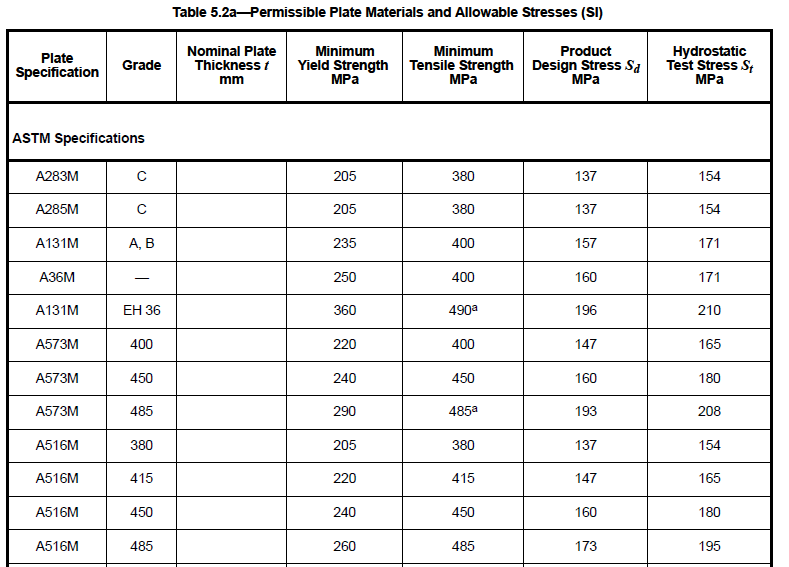
\includegraphics[width=1\linewidth]{fig/api650materiales}
	\label{fig:api650materiales}
\end{figure}

\section{Cálculo de cargas mayoradas}
Una carga mayorada es aquella que se multiplicada por un factor para aumentar su valor. En la ingeniería civil se suele mayorar las cargas según

\[
1,2 P_p + S_c + 1,6W
\]
donde $P_p$ es el peso propio de la estructura, $S_c$ es la sobrecarga de uso y $W$ son las cargas dinámicas (viento)

\section{Estructuras de acero para edificios[CIRSOC 301-2005]}
Este Reglamento es de aplicación a todos los elementos estructurales resistentes de
acero, laminados o armados con perfiles laminados y/o chapas, y sus uniones, que
formen parte de las estructuras de acero de edificios destinados a vivienda, locales
públicos, depósitos e industrias (incluso las que tengan carácter provisorio como
andamios cimbras, puntales, etc.), y que sean necesarias para soportar los efectos de
las acciones actuantes. Se incluyen las vigas carril de puentes grúas, monorrieles y las
estructuras de soporte de instalaciones y cañerías.

\subsection{Límites de esbeltez[B.7]}
\[
\text{Esbeltez} = \frac{kL}{r}
\]

\begin{description}
	\item[Barras comprimidas] la esbeltez será menor o igual que 200. En presencia de efectos dinámicos (como viento) se reduce a 150
	\item[Barras traccionadas] la esbeltez será menor o igual que 300. No aplica para cables.  En presencia de efectos dinámicos se reduce a 250. 
\end{description}

\subsection{Estabilidad de estructura[C.2]}

\begin{description}
	\item[Estruc. trianguladas interiormente isostaticas] $k = L_1/L$ donde $L_1$ es la distancia entre puntos no desplazables lateralmente por efecto del sistema de arriostramiento lateral, en cm. $L$ es la longitud real de la barra en cm
	\item[En pórticos y reticulados] cuya estabilidad lateral es provista por un sistema de
	arriostramiento, el factor de longitud efectiva $k$ para barras comprimidas se deberá tomar
	igual a la unidad, a menos que un análisis estructural demuestre que se puede adoptar un valor menor.
\end{description}


\subsection{Columnas (inestabilidad)[E.1]}
Son elementos sometidos a compresión con excentricidad. 

La resistencia de diseño para pandeo flexional:

\[
\phi_c P_n
\]
\begin{itemize}
	\item[$\phi_c$] = 0,85
	\item[$P_n$:] resistencia nominal, en kN. $P_{n}=F_{c r} A_{g}\left(10^{-1}\right)$ 
\end{itemize}

\[
F_{c r}=\begin{cases}
\left(0,658^{\lambda_{c}^{2}}\right) F_{y} & \lambda_c\leq 1,5 \\
\left( \frac{0,877}{\lambda_{c}^{2} } \right) F_{y} & \lambda_c > 1,5 \\
\end{cases} 
\]
\begin{itemize}
	\item[$F_y$:] Tensión de fluencia especificada, en MPa 
	\item[$A_g$:] Área bruta de barra, en cm$^2$
	\item[$\lambda_c$:] factor de esbeltez adimensional
	\[
	\lambda_{c}=\frac{1}{\pi} \frac{k L}{r} \sqrt{\frac{F_{y}}{E}}
	\] 
	\item[$E$:] Módulo de elasticidad longitudinal, en MPa
	\item[$k$:] Factor de longitud efectiva calculado según [C.2]
	\item[$L$:] Longitud real de la barra, en cm
	\item[$r$:] Radio de giro de la sección en cm
	\[
	r = \sqrt{ I/A_g }
	\]
	\item[$I$:] El segundo momento de inercia de la sección bruta, en cm$^4$
\end{itemize}

\subsection{Dimensionamiento de vigas al corte[F.2]}
El área del alma $A_w$ será el producto entre altura total de la sección $d$ por el espesor del alma $t_w$.

La resistencia de diseño al corte de almas no rigidizadas, con $h/t_w \leq 260$, será:
\[
\phi_v V_n
\]
\begin{itemize}
	\item[$\phi_v$] = 0,90
	\item[$V_n$:] La resistencia nominal al corte definido según las siguientes expresiones, en kN:
	\[
	\!\!\!\!\!\!\!\!V_n = \begin{dcases}
	\arraycolsep=1.4pt\def\arraystretch{2.2}
	0,6F_{yw} A_w (10^{-1})   \\
	\frac{0,6 F_{y w} A_{w}(2,45 \sqrt{E / F_{y w}})\left(10^{-1}\right)}{\left(h / t_{w}\right)} \\
	\frac{4,52 E A_{w}(10)^{-1}}{\left(h / t_{w}\right)^{2}}
	\end{dcases}
	\]	 
	Para los casos (respectivamente)
	\[
	\begin{cases}
	
	 \frac{h}{t_w}\leq 2,45 \sqrt{\frac{E}{F_{yw}}}\\
	 2,45\sqrt{\frac{E}{F_{yw}}}<\frac{h}{t_w}\leq 3,07 \sqrt{\frac{E}{F_{yw}}} \\
	 3,07 \sqrt{\frac{E}{F_{y w}}}<\frac{h}{t_{w}} \leq 260
	\end{cases}
	\]
	
	\item[$F_{yw}$:] Tensión de fluencia, en MPa 
	\item[$h$:] Distancia libre entre alas, unidades de $t_w$ [K.1.5]
\end{itemize}

\subsection{Uniones [J]}

\subsection{Resistencia a la tracción o al corte [J.3.6]}
La resistencia de diseño a la tracción o al corte de los bulones de alta resistencia y de elementos roscados será:
\[
\phi F_n A_b (10^{-1})
\]
\begin{itemize}
	\item[$\phi$:] el factor de resistencia indicado en la Tabla J.3.2.
	\item[$F_n$:] la resistencia nominal a la tracción Ft, o al corte Fv, indicadas en la Tabla J.3.2. , en MPa.
	\item[$A_b$:] el área nominal del cuerpo no roscado del bulón o de la parte roscada (para varillas recalcadas, ver la nota (c) al pie de la Tabla J.3.2.). ,en cm2.
\end{itemize}

\subsubsection{Combinación de tracción y corte en uniones tipo aplastamiento[J.3.7]}
La resistencia de diseño a tracción de un bulón sometido a corte y tracción
combinados será:
\[
\phi F_t A_b (10^{-1})
\]

\begin{itemize}
	\item[$\phi$:] = 0,75
	\item[$F_t$:] la resistencia nominal a tracción en términos de tensión calculada con las expresiones de la Tabla J.3.5. como una función de la tensión de corte requerida $f_v$ producida por las cargas mayoradas, en MPa. La tensión de corte requerida $f_v$ será menor o igual que la resistencia de diseño al corte $\phi F_v$ ,indicada en la Tabla J.3.2.  
\end{itemize}

\subsubsection{Bulones de alta resistencia en uniones de deslizamiento crítico[J.3.8]}
La resistencia de diseño al corte de bulones de alta resistencia en uniones de deslizamiento crítico se obtendrá de acuerdo con la Sección J.3.8(a) o J3.8(b). Los bulones así dimensionados se deberán verificar a corte trabajando en uniones tipo aplastamiento con las Secciones J.3.6. y J.3.7. y será verificado el aplastamiento de la chapa de acuerdo con las Secciones J.3.1. y J.3.10..

La\textbf{ resistencia de diseño al deslizamiento} $\phi R_\str$, deberá ser mayor o igual que la fuerza requerida debida a las cargas mayoradas, donde:
\[
R_{\str} = 1,13 \mu T_b N_s
\]

\begin{itemize}
	\item[$R_{\str}$:] la resistencia nominal al deslizamiento, en kN.
	\item[$T_b$:] la fuerza de tracción mínima del bulón dada en la Tabla J.3.1., en kN.
	\item[$N_s$:] la cantidad de superficies de rozamiento.
	\item[$\mu$:] el coeficiente medio de rozamiento para las Clases A, B, o C, según	corresponda, o el que surja de ensayos.
	\begin{itemize}
		\item[(a)] Para superficies Clase A (superficies de acero limpias con cepillo	metálico libres de polvo, óxido o cascarillas de laminación y no pintadas, o superficies con recubrimientos Clase A en acero limpiado con chorro de arena), $\mathbf{\mu=0,33}$
		\item[(b)] Para superficies Clase B (superficies de acero limpiadas con chorro de arena y no pintadas o superficies con recubrimiento Clase B en acero limpiado con chorro de arena), $\mathbf{\mu=0,50}$
		\item[(c)] Para superficies Clase C (superficies galvanizadas por inmersión en caliente y con superficies ásperas), $\mathbf{\mu=0,35}$
	\end{itemize}
\item[$\phi$] el factor de resistencia
\begin{itemize}
	\item[$\phi=1,0$] Para agujeros normales
	\item[$\phi=0,85$] 	Para agujeros holgados y ovalados cortos
	\item[$\phi=0,7$] Para agujeros ovalados largos con eje mayor perpendicular a la dirección de la fuerza
	\item[$\phi=0,6$] Para agujeros ovalados largos con eje mayor paralelo a la dirección de la fuerza
\end{itemize}
\end{itemize}

\subsubsection{Tracción y corte combinados en uniones de deslizamiento crítico[J.3.9]}
Cuando las uniones de deslizamiento crítico estén solicitadas por una fuerza de tracción $T_u$, que reduzca la fuerza de apriete entre las superficies en contacto, la \textbf{resistencia de diseño al rozamiento} $\phi R_\str$ de la Sección J.3.8(a) deberá ser multiplicada por
el siguiente factor, en el cual $T_u$ (kN) es la resistencia a tracción requerida bajo cargas mayoradas:
\[
[1 - T_u /(1,13 T_b N_b)]
\]
\begin{itemize}
	\item[$T_b$:] la fuerza de tracción mínima del bulón dada en la Tabla J.3.1., en kN.
	\item[$N_b$:] la cantidad de bulones cargados con la fuerza de tracción $T_u$.
\end{itemize}

\subsubsection{Resistencia al aplastamiento de la chapa en los agujeros[J.3.10]}
La resistencia al aplastamiento de la chapa será verificada tanto para las uniones tipo aplastamiento como para las tipo deslizamiento crítico. La utilización de agujeros holgados y ovalados cortos y largos con eje mayor paralelo a la dirección de la fuerza se restringe para las uniones de deslizamiento crítico por medio de la Sección J.3.2..

La \textbf{resistencia de diseño al aplastamiento de la chapa en los agujeros} será:
\[
\phi R_n
\]

\begin{itemize}
	\item[$\phi$] = 0,75
	\item[$R_n$:] la resistencia nominal al aplastamiento de la chapa, en kN.
\end{itemize}

\begin{figure}[htb!]
	\centering
	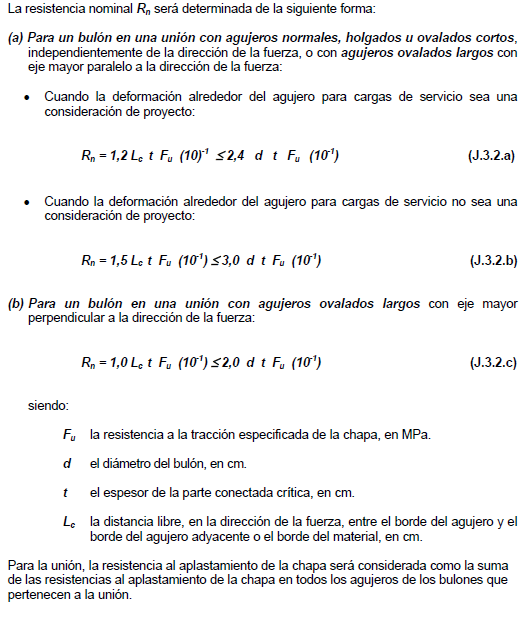
\includegraphics[width=1.13\linewidth]{fig/resistchapas.PNG}
\end{figure}











%%%%%%%%%%%%%%%%%%%%%%%%%%%%%%%55
%%
%%%%%%%%%%%%%%%%%%%%%%%%%%%%%%%%
\begin{figure}[htb!]
	\centering
	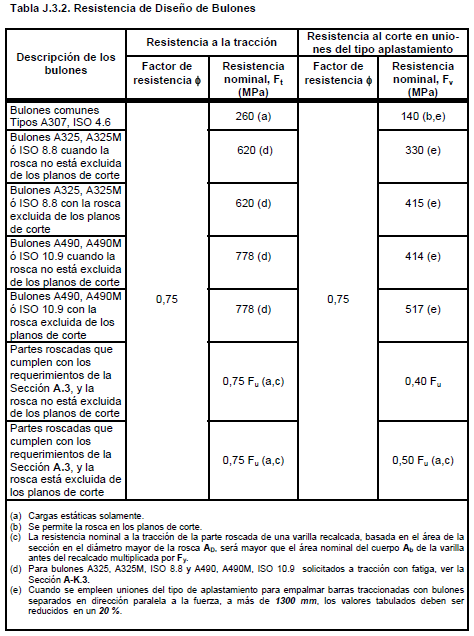
\includegraphics[width=1.1\linewidth]{fig/tabJ32.PNG}
\end{figure}

\begin{figure*}[htb!]
	\centering
	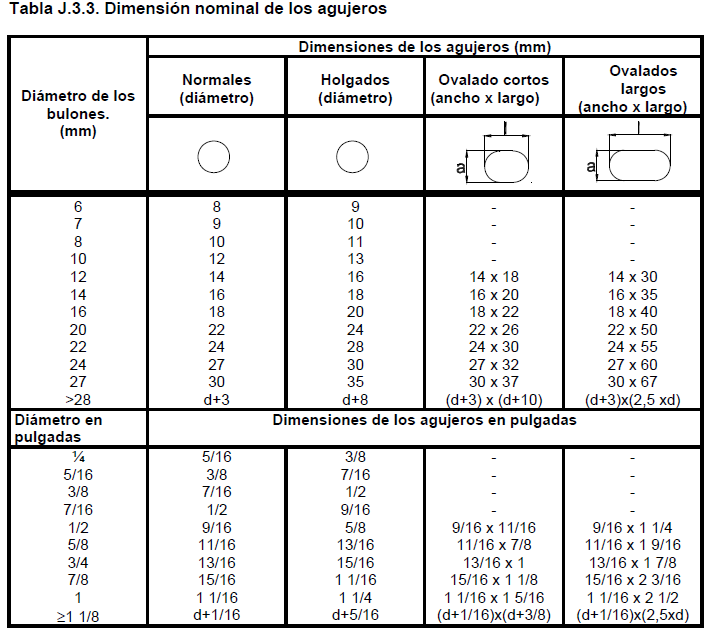
\includegraphics[width=\textwidth]{fig/tabJ33.PNG}
\end{figure*}

\begin{figure}[htb!]
	\centering
	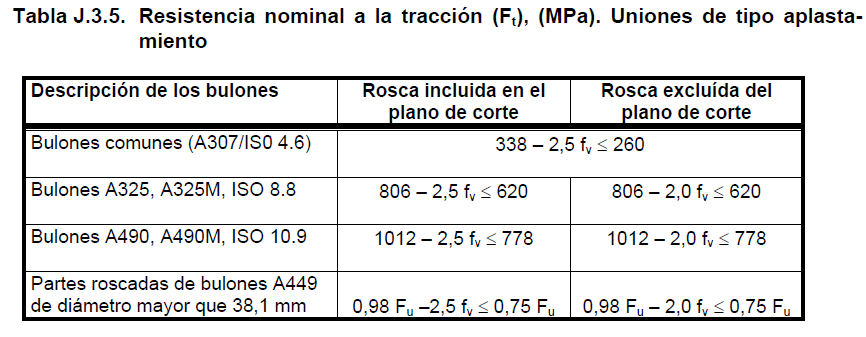
\includegraphics[width=1.1\linewidth]{fig/tabJ35.PNG}
\end{figure}








\clearpage
\subsection{Uniones [Apéndice J]}
\subsubsection{Resistencia al aplastamiento}
La resistencia de las superficies solicitadas al aplastamiento será:
\[
\phi R_n
\]
\begin{itemize}
	\item[$\phi$] = 0,75
	\item[$R_n$] la resistencia nominal al aplastamiento, en kN
\end{itemize}
donde
\begin{itemize}
	\item Para superficies mecanizadas, pernos pasantes en agujeros escariados, taladrados
	o punzonados y en los extremos de rigidizadores ajustados trabajando a
	aplastamiento:
	\[
R_n = 1,8 F_y A_{pb} (10^{-1})
\]
\item[$F_y$:] la tensi\'on de fluencia especificada, en MPa
\item[$A_{pb}$:] la proyecci\'on del \'area
\end{itemize}
\subsubsection{Bulones (desl. crítico)}

\begin{table*}[htb!]
	\centering
	\caption{\textbf{A-J.3.1.} Resistencia nominal a la tracción ($F_t$), en MPa. Uniones de tipo aplastamiento.}
%	\footnotesize
	\begin{tabular}{|c|c|c|}
		\hline 
		\thead{Descripción de \\ los bulones} & \thead{Rosca incluída\\ en el
		plano\\ de corte} & \thead{Rosca excluída \\ del
		plano\\ de corte} \\ 
		\hline 
		\thead{Bulones Comunes\\
		Tipo A307, ISO 4.6} & \multicolumn{2}{c|}{$\sqrt{620^{2}-6,25 f_{v}^{2}}$} \\ 
		\hline 
		\thead{Bulones
		A325,\\ A325M
		ISO 8.8} & $\sqrt{620^{2}-6,25 f_{v}^{2}}$ & $\sqrt{620^{2}-4.00f_{v}^{2}}$ \\ 
		\hline 
		\thead{Bulones
		A490,\\ A490M
		ISO 10.9} & $\sqrt{778^{2}-6,42 f_{v}^{2}}$ & $\sqrt{778^{2}- 4,04 f_{v}^{2}}$ \\ 
		\hline 
		\thead{Partes roscadas de\\
		bulones A449 de\\
		diámetro mayor\\ que
		38.1 mm} & $\sqrt{(0,75F_u)^{2}-6,25 f_{v}^{2}}$ & $\sqrt{(0,75F_u)^{2}-4,00 f_{v}^{2}}$ \\ 
		\hline 
	\end{tabular} 
\end{table*}

Según \textbf{A-J.3.8(b). Uniones de deslizamiento crítico dimensionadas para cargas de servicio}, a resistencia de diseño al corte de un bulón en una unión de deslizamiento crítico para cargas de servicio será:

\[
\phi F_v A_b (10^{-1})
\]
\begin{itemize}
	\item[$\phi$] = 1,0  para agujeros normales, holgados, ovalados cortos, y ovalados largos	cuando el eje más largo es perpendicular o paralelo a la línea de fuerza.
	\item[$F_v$:] la resistencia al deslizamiento crítico para cargas de servicio indicada en 
	Tabla A-J.3.2, en MPa
	\item[$A_b$:] área nominal del cuerpo no roscado del bulón, o de la parte roscada, en cm$^2$. 
\end{itemize}

\textbf{A-J.3.9(b). Uniones de deslizamiento crítico dimensionadas para cargas de servicio}.
La resistencia de diseño al corte de un bulón en una unión de deslizamiento crítico
solicitada a una fuerza de tracción T (kN) debida a las cargas de servicio que reduce la
fuerza de apriete entre las partes en contacto, será $\phi F_v A_b$ (10-1), calculada de acuerdo con
lo especificado en la Sección A-J.3.8(b) multiplicada por el siguiente factor de reducción :

 \[
 1 - \frac{T}{0,8T_b N_b}
 \]
 
 \begin{itemize}
 	\item[$T_b$:] El pretensado mínimo del bulón dado por tabla A-J.3.1, en kN
 	\item[$N_b$:] el número de bulones cargados con la tracción de servicio $T$, en kN
 \end{itemize}




\begin{table}[htb!]
	\centering
	\caption{\textbf{A-J.3.2.} Resistencia al corte Fv para cargas de servicio de bulones de alta
		resistencia en uniones de deslizamiento crítico (a) (MPa).}
	\footnotesize
	\begin{tabular}{|c|c|c|c|}
		\hline 
		\thead{Tipo de \\ bulón}&\thead{Agujeros\\normales}  & \thead{Agujeros\\holgados y\\ovalados\\ cortos} & \thead{Agujeros\\ ovalados\\ largos\\perpendicular\\ (paralelo) a linea\\ de fuerza} \\ 
		\hline 
		\thead{A325,\\ A325M\\ISO 8.8}	& 117 & 103 & 83 (69) \\ 
		\hline 
		\thead{A490,\\ A490M\\ISO 10.9}	& 145 & 124 & 103 (90)  \\ 
		\hline 
	\end{tabular} 
\end{table}




\clearpage
\section{Dimensionado de elementos con armadura}
Caso de carga básico
\[
1,2P_p +S_c + 1,6W
\]
El momento último de servicio (trasladando al baricentro de la armadura) es
\[
M_{us} = M_{mayorada} - N(d-h/2)
\]
considerar pretensado sobre $N$.
\subsection{Predimensionado de columna ante compresión}

Para poder emplear métodos aproximados se plantea la siguiente desigualdad

\[
h > \sqrt[3]{  \frac{24 \cdot n \cdot P_u (kz\ell_u)^2}{ b E_c}  }
\]
donde $n$ es el factor de sobredimensionamiento (siempre mayor a 1). 
\section{Estructuras de hormigón[CIRSOC 201-2005]}

\subsection{Módulo de elasticidad [8.5]}

8.5.1. El módulo de elasticidad $E_c$ del hormigón de densidad normal (entre 2000 y 2800 $\text{kg/m}^3$) se puede determinar con la expresión (8-1) siempre que las tensiones no superen el valor $0,45\sqrt{f'_c}$ :

\[
E_c = 4700 \sqrt{f'_c} \qquad \text{(en MPa)}
\]

8.5.2. El módulo de elasticidad $E_s$ de la armadura no tesa, se puede considerar igual a:
\[
E_s = 200000 \text{MPa} = 200 \text{GPa}
\]

\subsection{Requisitos generales [9.1]}
9.1.1. Las estructuras y los elementos estructurales se deben diseñar para obtener,
en cualquier sección, una resistencia igual o mayor que la resistencia requerida, determinada para las cargas mayoradas combinadas en la forma establecida en este
Reglamento.

El requisito básico para el diseño por resistencia de estructuras de hormigón se
puede expresar de la siguiente forma:
\begin{IEEEeqnarray*}{uc.s}
Resistencia de Diseño & \geq & Resistencia Requerida \\
$\phi S_n$ &\geq & $U$
\end{IEEEeqnarray*}
donde $U$ es la resistencia requerida para resistir las cargas mayoradas o las solicitaciones
correspondientes y $S_n$ es la resistencia nominal en N.

9.3.2. El factor de reducción de resistencia $\phi$, para aquellas combinaciones que no
incluyen sismo, debe ser el indicado en los artículos 9.3.2.1. al 9.3.2.5. inclusive (siguientes puntos):

\begin{description}
	\item[$\phi = 0,90$] Para secciones controladas por traccion segun 10.3.4
	\item[$\phi=0,65$] Secciones controladas por compresión según 10.3.3
\end{description}


\subsection*{Campo de validez del capítulo 10}
Este Capítulo se debe aplicar al diseño de elementos solicitados a flexión o por cargas axiales, o por una combinación de flexión y cargas axiales.
\subsection{Nomenclatura Capítulo 10}
\begin{description}
	\item[$a$] altura del bloque de tensiones rectangular equivalente, definido en el artículo 10.2.7.1., en mm.
	\item[$A_s,A_{st}$] Area de la armadura longitudinal traccionada no tesa en mm$^2$
	\item[$A_g$] área total o bruta de la sección. En una sección hueca, Ag es el área de
	hormigón solamente, en mm$^2$
	\item[$b$] ancho del borde comprimido de la sección transversal de un elemento, en mm.
	\item[$b_w$] Alto de alma para un elemento con alas, en mm$^2$
	\item[$c,c_t$] distancia desde la fibra comprimida extrema al eje neutro, en mm.
	\item[$h$] espesor o altura total de la sección transversal de un elemento, en mm
	\item[$d$] distancia desde la fibra comprimida extrema hasta el baricentro de la armadura longitudinal traccionada, no tesa, (altura útil), en mm$^2$
	\item[$d_t$] distancia desde la fibra comprimida extrema hasta el baricentro de la capa de armadura longitudinal más traccionada, en mm.
	\item[$E_c$] módulo de elasticidad del hormigón, en MPa. Ver el artículo 8.5.1.
	\item[$E_s$] módulo de elasticidad de la armadura no tesa, en MPa. Ver el artículo 8.5.2.
	\item[$C_m$] factor que relaciona el diagrama real de momentos con un diagrama equivalente de momentos uniforme.
	\item[$k$] factor de longitud efectiva para elementos comprimidos.
	\item[$I_g$] momento de inercia de la sección total o bruta del elemento de hormigón con respecto al eje baricéntrico, sin considerar la armadura, en mm$^4$.
	\item[$f_c'$] resistencia especificada a la compresión del hormigón, en MPa. $\sqrt{f_c'}$ también es en MPa
	\item[$f_y$] tensión de fluencia especificada de la armadura longitudinal no tesa, (corresponde
	al límite de fluencia de la norma IRAM-IAS), en MPa.
	\item[$\ell_u$] longitud sin apoyo lateral de un elemento comprimido, en mm. Ver el artículo 10.11.3.1.
	
	\item[$M_c$] momento mayorado debido a las cargas que producen un desplazamiento horizontal apreciable, en N mm.
	\item[$M_s$] momento mayorado debido a las cargas que producen un desplazamiento horizontal apreciable, en N mm.
	\item[$M_u$] momento mayorado en la sección considerada, en N mm.
	\item[$M_1$] el menor momento (de primer orden), mayorado en uno de los extremos de un elemento comprimido, que se debe adoptar como positivo si el elemento presenta curvatura simple, y negativo si tiene doble curvatura, en N mm
	\item[$M_2$] el mayor momento (de primer orden) mayorado, en uno de los extremos de un elemento comprimido, siempre positivo, en N mm
	\item[$M_{1ns}$] momento mayorado de un elemento comprimido, en el extremo en el cual actúa $M_1$, debido a cargas que no originan desplazamiento lateral apreciable, y calculado mediante un análisis elástico de primer orden del pórtico, en N mm.
	\item[$M_{1s}$] momento mayorado de un elemento comprimido, en el extremo en el cual actúa $M_1$, debido a cargas que originan un desplazamiento lateral apreciable, y calculado mediante un análisis elástico de primer orden del pórtico, en N mm.
	
	
	\item[$P_b$] resistencia nominal para carga axial (resistencia axial nominal) en la condición de deformación balanceada, en N. Ver el artículo 10.3.2.
	\item[$P_c$] carga crítica de pandeo, en N. Ver el artículo 10.12.3.
	\item[$P_n$] resistencia nominal para la carga axial, (resistencia axial nominal) de la sección transversal, en N.
	\item[$P_u$] esfuerzo axial mayorado para una excentricidad dada ($P_u \leq \phi P_n$), en N. Se debe considerar positivo para compresión y negativo para tracción.
	\item[$Q$] índice de estabilidad de un piso. Ver el artículo 10.11.4.
	\item[$\beta_d$] relación utilizada para calcular los momentos amplificados en las columnas
	debidos a las cargas sostenidas o de larga duración. Ver los artículos 10.11.1. y
	10.13.6.
	\item[$\beta_1$] factor que relaciona la altura del bloque de tensiones de compresión rectangular
	equivalente con la profundidad del eje neutro. Ver el artículo 10.2.7.3.
	\item[$\delta_{ns}$] factor de amplificación de momentos para pórticos indesplazables, utilizado para
	reflejar los efectos de la curvatura entre los extremos del elemento comprimido.
	\item[$\delta_s$] factor de amplificación de momentos para pórticos desplazables, utilizado para
	reflejar el desplazamiento lateral que resulta de las cargas gravitatorias y de las
	cargas laterales.
	\item[$\Delta_o$] desplazamiento lateral relativo entre el extremo superior e inferior de un piso
	debido a los esfuerzos horizontales, calculado mediante un análisis elástico de
	primer orden del pórtico, con valores de rigideces que satisfagan lo especificado
	en el artículo 10.11.1.
	\item[$\varepsilon_t$] deformación específica neta de tracción en el acero más traccionado para la
	resistencia nominal, excluyendo las deformaciones debidas a la tensión efectiva del pretensado, la fluencia lenta, la contracción y las variaciones de temperatura.
	\item[$\rho$] cuantía de la armadura traccionada, no tesa; relación entre $A_s$ y $b d$, ($\rho = A_s /b d$). Ver el artículo C 10.3.3. y el Apéndice B.
	\item[$\rho_b$] cuantía de la armadura que produce condiciones de deformación balanceadas;	relación entre $A_s$ y $b d$ ($\rho_b = A_s/b d$). Ver el artículo 10.3.2.
	\item[$\phi$] factor de reducción de la resistencia. Ver el artículo 9.3.
\end{description}
\subsection{Hipótesis de diseño [10.2]}
10.2.1. El diseño por resistencia de elementos solicitados a flexión y cargas axiales se
debe fundamentar en las hipótesis establecidas en los artículos 10.2.2. a 10.2.7. inclusive y debe satisfacer las condiciones de equilibrio y de compatibilidad de las
deformaciones.

10.2.2. Las deformaciones específicas en la armadura y en el hormigón se deben suponer directamente proporcionales a la distancia al eje neutro, excepto en vigas de gran altura

10.2.3. Para la determinación de la resistencia nominal de una sección, se debe considerar como máxima deformación en la fibra extrema del hormigón sometida a
compresión un valor igual a 0,003.

10.2.4. La tensión en el acero se debe calcular como Es veces la deformación de la armadura, siempre que dicha tensión resulte menor que la tensión de fluencia especificada fy . Para deformaciones mayores que la correspondiente a fy , la tensión se debe considerar independiente de la deformación, e igual a fy .

10.2.5. La resistencia a la tracción del hormigón no se debe considerar en el dimensionamiento de los elementos de hormigón armado solicitados a flexión y a cargas axiales, excepto cuando se cumplan los requisitos del artículo 18.4.

10.2.6. La relación entre la tensión de compresión en el hormigón y la deformación específica del hormigón, se debe suponer rectangular, trapezoidal, parabólica, o de
cualquier otra forma que dé origen a una predicción de la resistencia que coincida en forma sustancial con los resultados de ensayos.

10.2.7. Los requisitos del artículo 10.2.6. se satisfacen con una \textbf{distribución rectangular equivalente} de tensiones en el hormigón, definida en los artículos 10.2.7.1. a 10.2.7.3. inclusive.

10.2.7.1. La tensión en el hormigón se adopta igual a 0,85 f’c , y se supone uniformemente distribuida en una zona de compresión equivalente, limitada por los
extremos de la sección transversal, y por una línea recta paralela al eje neutro, a una distancia $a = \beta_1 c$, a partir de la fibra comprimida con deformación máxima.

10.2.7.2. La distancia c, entre la fibra comprimida con deformación máxima y el eje
neutro, se debe medir en dirección perpendicular a dicho eje.

10.2.7.3. Como valor del factor $\beta_1$ se debe adoptar:
\begin{IEEEeqnarray*}{tc}
para $f'_c \leq 30$ MPa & \beta_1 = 0,85 \\
para $f'_c > 30$ MPa & \beta_{1}=0,85-0,05 \frac{\left(f_{c}^{\prime}-30 M P a\right)}{7}
\end{IEEEeqnarray*}
siempre que $\beta_1>0,65$

\subsection{Principios  y requisitos generales [10.3]}
10.3.1. El diseño de una sección transversal solicitada a cargas axiales o a flexión, o a una combinación de ambas (flexocompresión), se debe basar en la \textbf{compatibilidad de tensiones y deformaciones}, utilizando las hipótesis establecidas en el artículo 10.2.

10.3.2. La condición de deformación balanceada se define como aquella situación que se produce en una sección transversal cuando la deformación en la armadura traccionada es la correspondiente a la tensión de fluencia especificada $f_y$ , y en la fibra comprimida con
deformación máxima la deformación específica es igual al valor último ($\varepsilon_t =$ valor último), adoptado igual a 0,003.

10.3.3. Las secciones son controladas por compresión cuando la deformación neta por tracción en el acero más traccionado, $\varepsilon_t$ , es igual o menor que la deformación límite controlada por compresión ($ \varepsilon_t = f_y /E_s$), y en el hormigón comprimido la deformación específica es igual al valor último, adoptado igual a 0,003 .

La deformación límite controlada por compresión es la deformación específica neta de tracción en la armadura, en condiciones de deformación balanceada.
Para la armadura fy = 420 MPa y para todas las armaduras pretensadas, se permite fijar el límite de la deformación controlada por compresión en un valor igual a 0,002.

10.3.4. Las secciones son controladas por tracción cuando la deformación neta por
tracción en el acero más traccionado, $\varepsilon_t$ , es igual o mayor que 0,005 y en el hormigón comprimido la deformación específica es igual al valor último, adoptado igual a 0,003.

Las secciones con una deformación neta por tracción en el acero más traccionado, $\varepsilon_t$ , comprendida entre la deformación límite controlada por compresión ( $\varepsilon_t = f_y /E_s$) y el valor
0,005, corresponden a una región de transición entre las secciones controladas por compresión y aquellas controladas por tracción.

10.3.5. Para los elementos no pretensados solicitados a flexión y para los elementos no pretensados solicitados por una carga de compresión axial mayorada menor que $0,10 f'_c A_g, (\phi P_n \leq 0,10 f'_c A_g )$, la deformación neta de tracción, $\varepsilon_t$ , para la resistencia
nominal debe ser igual o mayor que 0,004.

\textbf{10.3.6.} La resistencia de diseño a carga axial, $\phi P_n$ , de los elementos comprimidos, debe ser igual o menor que $\phi P_{n,\max}x$ , determinada mediante las expresiones (10-1) ó (10-2).

10.3.6.2. Para elementos no pretensados armados con estribos cerrados, que cumplan con el artículo 7.10.5. (columnas), se debe utilizar:

\[
\phi P_{n, \max }=0,80 \phi\left[0,85 f'_{c}\left(A_{g}-A_{s t}\right)+f_{y} A_{s t}\right]
\]
Ver código para elementos pretensados o con zunchos en espiral.

10.3.7. Los elementos solicitados por una carga axial de compresión se deben diseñar para el momento máximo que pueda acompañar a dicha carga axial. La carga axial mayorada, $P_u$ , para una excentricidad dada, no debe exceder el valor de la resistencia de diseño a carga axial, $\phi P_n$ , especificada en el artículo 10.3.6. El momento máximo mayorado, $M_u$ , se debe incrementar por los efectos de la esbeltez, de acuerdo con las especificaciones del artículo 10.10.


\subsection{Armadura mínima en elementos solicitados a flexión [10.5]}

10.5.1. El área As adoptada en cada sección de un elemento solicitado a flexión, en el
que se requiera por cálculo armadura de tracción, con excepción de los casos definidos
en los artículos 10.5.2., 10.5.3. y 10.5.4., debe ser como mínimo:

\[
A_{s, \min }=\frac{\sqrt{f^{\prime}_c}}{4 f_{y}} b_{w} d \quad \text{siempre que} \quad A_{s, \min } \geq \frac{1,4 b_{w} d}{f_{y}}
\]

\subsection{Límites para la armadura de elementos comprimidos [10.9]}
10.9.1. El área de armadura longitudinal, $A_{st}$ , para elementos comprimidos no
compuestos, debe ser:

\[
0,01A_g \leq A_{st} \leq 0,08 A_g
\]
\subsection{Momentos amplificados - Conceptos generales}

10.11.1. Las fuerzas axiales mayoradas, $P_u$ , los momentos mayorados $M_1$ y $M_2$ en los extremos de la columna y, cuando se requiera, la deformación lateral de piso, $\Delta_o$ , se
deben calcular por medio de un análisis elástico de primer orden del pórtico, considerando
el efecto de las cargas axiales, la presencia de zonas fisuradas a lo largo del elemento y
los efectos de la duración de las cargas en las propiedades de la sección. Como
alternativa, se permiten utilizar para los elementos de la estructura las propiedades que se
especifican en la Tabla 10.11.1.

\subsection{Momentos amplificados - Pórticos indesplazables [10.12]}

10.12.1 Para los elementos comprimidos en pórticos indesplazables, el factor de
longitud efectiva $k$ debe ser igual a 1.

10.12.2. En los pórticos indesplazables se pueden ignorar los efectos de la esbeltez, en
aquellos elementos comprimidos que verifiquen la siguiente expresión

\[
\frac{k \ell_{u}}{r} \leq 34-12\left(\frac{M_{1}}{M_{2}}\right) \quad \text{con} \quad  34-12\left(\frac{M_{1}}{M_{2}}\right)=40 
\]

donde el término $M_1 / M_2$ es positivo si el elemento se deforma con curvatura simple
(momentos extremos de igual signo) y negativo si el elemento se deforma con
curvatura doble (momentos extremos de distinto signo). Ambos momentos son de primer orden.

10.12.3. Los elementos comprimidos se deben dimensionar para la carga axial
mayorada Pu y para el momento mayorado y amplificado por los efectos de la
curvatura del elemento, Mc , de acuerdo con las siguientes expresiones:

\[M_{c}=\delta_{n s} M_{2}\]
siendo 

\begin{IEEEeqnarray*}{cc}
\delta_{n s}  =&\frac{C_{m}}{1-\frac{P_{u}}{0,75 P_{c}}} \geq 1,0 \\
P_{c}  =&\frac{\pi^{2} E I}{\left(k \ell_{u}\right)^{2}} \\
EI=&\frac{0,2 E_{c} I_{g}+E_{s} I_{s e}}{1+\beta_{d}} \quad \text{ó} \\
EI=& {\frac{0,4 E_{c} I_g}{1+\beta_{d}}}
\end{IEEEeqnarray*}

Para pórticos \textbf{indesplazables}, $\beta_d$ , es la relación entre la máxima carga axial
mayorada que actúa en forma permanente (carga de larga duración) y la máxima carga axial mayorada asociada a la misma combinación de cargas.

Para pórticos \textbf{desplazables}, excepto en el caso especificado en el artículo
10.13.6., $\beta_d$ es la relación entre el máximo corte mayorado que actúa en forma  permanente (carga de larga duración) en un entrepiso y el corte máximo mayorado de ese entrepiso.


10.12.3.1. El coeficiente $C_m$ , para los elementos sin cargas transversales entre sus
apoyos, se debe obtener de la siguiente expresión:

\[
C_{m}=0,6+0,4 \frac{M_{1}}{M_{2}} \geq 0,4
\]
Para elementos con cargas transversales entre sus apoyos $C_m=1$

\subsection{Momentos amplificados - Pórticos desplazables [10.13]}
10.13.1. Para elementos comprimidos en pórticos desplazables, el factor de longitud
efectiva $k$, se debe determinar utilizando los valores de $E$ e $I$ indicados en el artículo
10.11.1/8.5, y debe ser \(k>1\)

10.13.2. En los elementos comprimidos desplazables, o sea no arriostrados contra el
desplazamiento lateral, se permite despreciar los efectos de la esbeltez, cuando se
verifique que \(k \ell_u / r <22\)

10.13.3. Los momentos $M_1$ y $M_2$ en los extremos de un elemento individual comprimido, se
deben obtener con las siguientes expresiones:

\begin{IEEEeqnarray*}{c}
M_1 = M_{1ns} + \delta _s M_{1s} \\
M_2 = M_{2ns}+\delta_s M_{2s}
\end{IEEEeqnarray*}
donde $\delta_s M_{1s}$ y $\delta_s M_{2s}$ se deben calcular de acuerdo con 10.13.4

\subsubsection{Determinación de $\delta_s M_s$ [10.13.4]}
10.13.4.1. Los momentos amplificados por efecto del desplazamiento lateral, $\delta_s M_s$ , se
deben considerar como los momentos extremos de la columna, determinados por medio
de un análisis elástico de segundo orden basado en las rigideces del elemento,
establecidas en el artículo 10.11.1.

10.13.4.2. En forma alternativa y sólo cuando las columnas del piso tengan igual altura, el
valor de $\delta_s M_s$ se podrá calcular con la siguiente expresión :
\[
\delta_{s} M_{s}=\frac{M_{s}}{1-Q} \geq M_{s}
\]
Si el valor de $\delta_s$ , determinado con la expresión (10-17), es $> 1,5$, entonces el valor $\delta_s M_s$
se debe calcular de acuerdo con lo indicado en los artículos 10.13.4.1. ó 10.13.4.3.

10.13.4.3. Otra forma de determinación consiste en calcular el momento amplificado por
desplazamiento lateral, $\delta_s M_s$ , con la siguiente expresión:

\[
\delta_{s} M_{s}=\frac{M_{s}}{1-\frac{\sum P_{u}}{0,75 \sum P_{c}}} \geq M_{s}
\]

\begin{description}
	\item[$\sum P_u$] la sumatoria de todas las cargas verticales mayoradas en un piso
	\item[$\sum P_c$] la sumatoria de las cargas de las columnas que resisten el desplazamiento
	lateral de un piso,
	\item[$P_c$] la carga crítica determinada con la expresión (10-10), utilizando para $k$ el
	valor indicado en el artículo 10.13.1.
\end{description}

10.13.7. En pórticos desplazables, los elementos solicitados a flexión se deben diseñar
para la totalidad de los momentos amplificados de los elementos comprimidos que
concurren al nudo.

\begin{figure*}[htb!]
	\centering
	\hspace{2cm}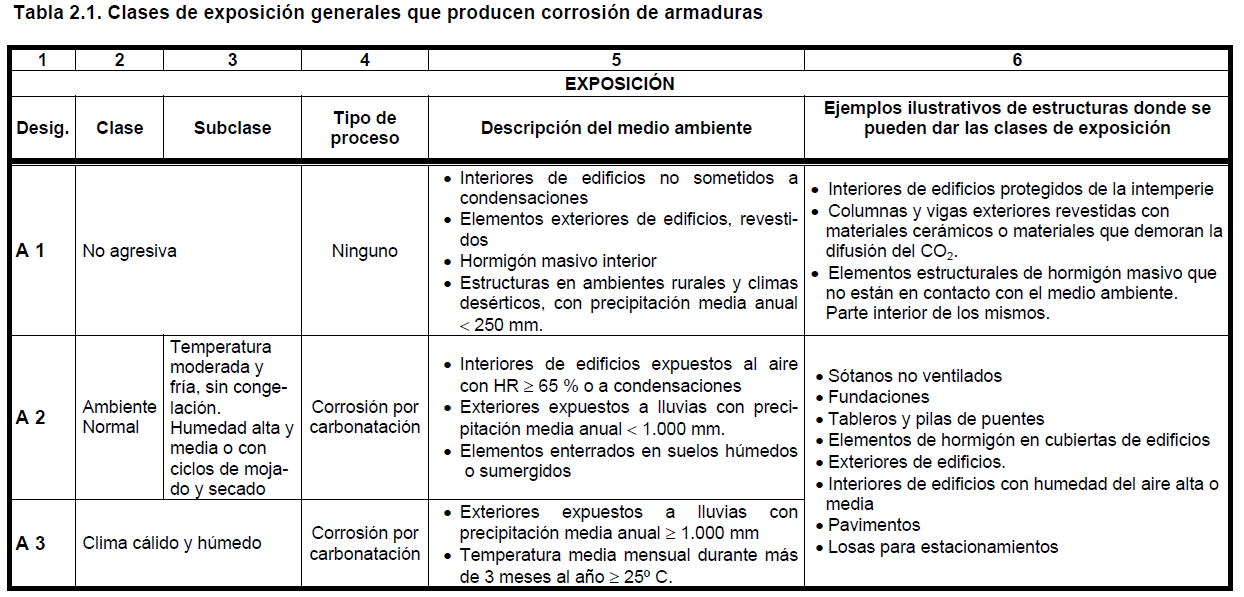
\includegraphics[width=1\linewidth]{fig/cirsoc201tab21}
	\label{fig:cirsoc201tab21}
\end{figure*}
\begin{figure*}
	\centering
	\hspace{2cm}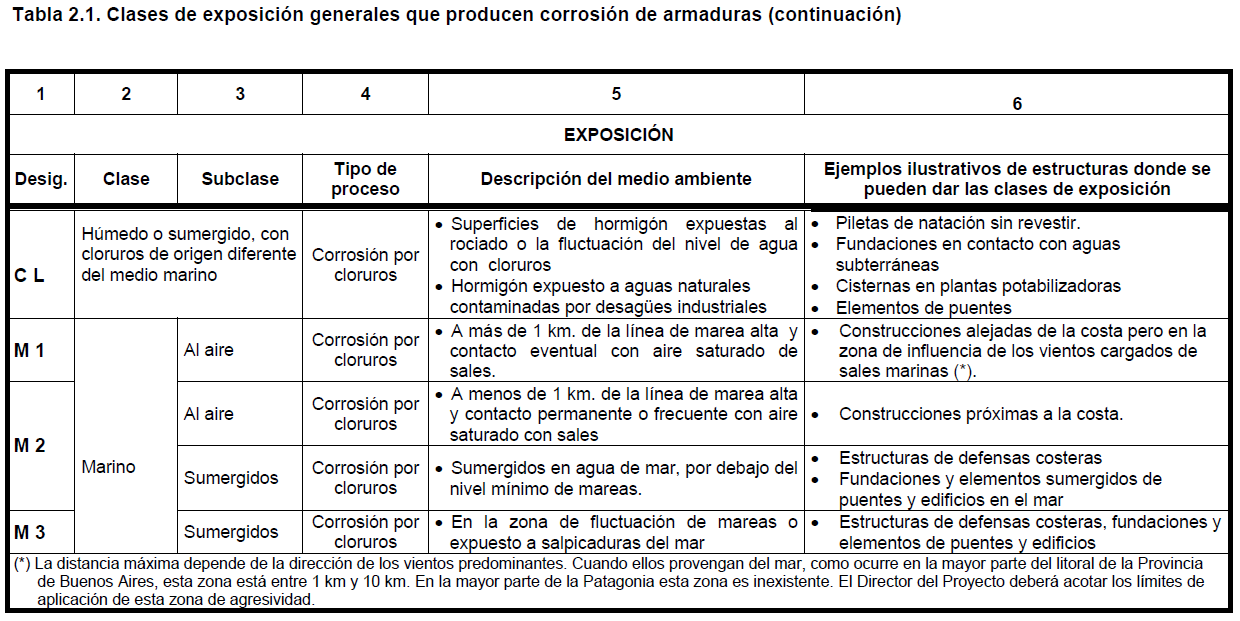
\includegraphics[width=1\linewidth]{fig/cirsoc201tab21c}
	\caption{CIRSOC 201}
	\label{fig:cirsoc201tab21c}
\end{figure*}

\begin{figure*}
	\centering
	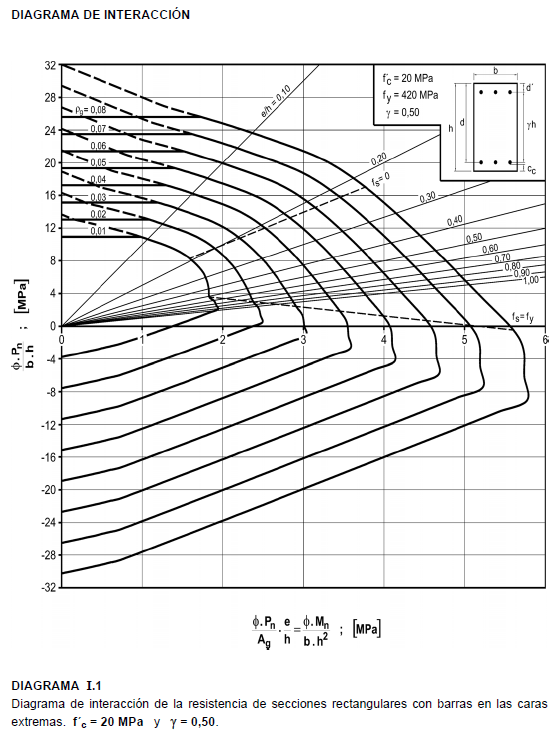
\includegraphics[width=1\linewidth]{fig/cirsoc102nomog1}
	\label{fig:cirsoc102nomog1}
\end{figure*}


\end{document}


\begin{itemize}
	\item[$y$:] 
	\item[$y$:] 
	\item[$y$:] 
\end{itemize}

 